\usepackage[utf8]{inputenc}	% Para caracteres en español
\usepackage{amsmath,amsthm,amsfonts,amssymb,amscd}
\usepackage{multirow,booktabs}
\usepackage[table]{xcolor}
\usepackage{fullpage}
\usepackage{lastpage}
\usepackage{enumitem}
\usepackage{fancyhdr}
\usepackage{mathrsfs}
\usepackage{wrapfig}
\usepackage{setspace}
\usepackage{hyperref}
\usepackage{calc}
\usepackage{multicol}
\usepackage{cancel}
\usepackage[retainorgcmds]{IEEEtrantools}
\usepackage[margin=3cm]{geometry}
\usepackage{amsmath}
\newlength{\tabcont}
\setlength{\parindent}{0.0in}
\setlength{\parskip}{0.05in}
\usepackage{empheq}
\usepackage{framed}
\usepackage[most]{tcolorbox}
\usepackage{xcolor}
\colorlet{shadecolor}{orange!15}
\parindent 0in
\parskip 12pt
\geometry{margin=1in, headsep=0.25in}
\theoremstyle{definition}
\usepackage{pdfpages}
\newtheorem{defn}{Definition}
\newtheorem{reg}{Rule}
\newtheorem{exer}{Exercise}
\newtheorem{note}{Note}
\usepackage{fancyhdr}\usepackage{xcolor}\usepackage{amsmath}\usepackage{amssymb}\pagestyle{fancy}\rhead{}
\newtheorem{theorem}{Theorem}[subsection]
\theoremstyle{definition}
\newtheorem{definition}[theorem]{Definiton}
\newtheorem{example}[theorem]{Example}
\newtheorem{corollary}[theorem]{Corollary}
\newtheorem{lemma}[theorem]{Lemma}
\title{Chapter 9 Review Notes}
\begin{document}

\thispagestyle{empty}
\begin{center}
{\LARGE \bf CIV 102 Notes}\\
{\large Hayson Cheung}\\
Structures and Materials, Fall 2024\\
\vspace{10pt}
\textit{"Structural Engineering is the art and science of designing and molding structures with economy and elegance so that they can safely resist the force that they are subjected''}
\end{center}
\section{Force, Moment, and Load} 
\subsection{Moment}
\begin{definition}[Moment]
    The moment is an object's tendency to rotate, measured in Newton-Meters (\textbf{Nm}).
\end{definition}
\begin{shaded}
    \paragraph{Force-Coupled Moment} Two forces act in \textbf{opposite directions} but the \textbf{same magnitude} creates force-coupled moment.
    \begin{equation}
        \mu = \mathrm{moment} = \Vec{F}\times\Vec{d}
    \end{equation}
    Where:
    \begin{equation*}
    \begin{split}
    \Vec{F} = \text{Coupled forces (N)} \\
    \Vec{d} = \text{Displacement between the coupled forces (m)} \\
    \end{split}
    \end{equation*}
    \\Note that the moment is calculated in the cross-products, and the direction of that vector is the axis of rotation,
    \end{shaded}
\paragraph{Signs} If the moments return a positive value, it is a counter-clockwise rotation, and vice versa. 
\paragraph{Static Equilibrium} The state in which the sum of all component forces, including moments, equals zero. (In civ, things are most likely not supposed to move, so this is used often)
\begin{equation}
    \sum F_x=0,\sum F_y=0, \sum \mu = 0
\end{equation}
\begin{shaded}
    \paragraph{Moment for One Force} The moment due to only one force is:
    \begin{equation}
        \mu = \mathrm{moment} = \Vec{F}\times\Vec{d_\perp}
    \end{equation}
Where:
\begin{equation*}
\begin{split}
\Vec{d_\perp} = \text{The perpendicular displacement to the center of rotation}
\end{split}
\end{equation*}
\end{shaded}
\subsection{Moment of Inertia}
\paragraph{} For Linear Force, we have:
$$
F=ma
$$
\begin{shaded}
    \paragraph{Mass-moment Inertia} Its counterpart in moment is the following
    \begin{equation}
        \mu = \mathrm{moment} = \omega\alpha
    \end{equation}
    Where:
    \begin{equation*}
    \begin{split}
    \omega = \text{Mass-Moment Inertia} \\
    \Vec{d} = \text{Rotational Acceleration} \\
    \end{split}
    \end{equation*}
\end{shaded}
\paragraph{}
\paragraph{} and for position, acceleration, and velocity:
\begin{equation}
    x = \theta y
\end{equation}
\begin{equation}
    \dot{x} = \dot{\theta} y
\end{equation}
\begin{equation}
    \ddot{x} = \ddot{\theta} y
\end{equation}
\paragraph{Multiple point Masses} 
\begin{equation}
    I_m = \Sigma_i y_i^2 m_i
\end{equation}
\paragraph{Distributed Mass} 
\begin{equation}
    I_m = \int y^2 d m
\end{equation}
\paragraph{} Let $\rho$ be the mass density, assume constant thickness, so $dm = \rho t dA$
\subsection{Hanging Cables}
\begin{equation}
    I_m = \rho t\iint y^2 dA
\end{equation}
$I = \iint y^2 dA$ is called the moment of inertia. For $I$ in a rectangle with the axis of rotation in its middle, $R$, we have.
\begin{equation}
    I = bh^3/12
\end{equation}
\begin{minipage}{0.55\textwidth}
\begin{definition} [Type I Hanging Cables]
    Cables under its weight, follow the shape of a \textbf{catenery}. It has \textbf{non-uniform} horizontal weight distribution. 
\end{definition}
\paragraph{} This is not a practical case as there certainly would always be loads other than the cable.
\end{minipage}
\begin{minipage}{0.05\textwidth}
    \hspace{\textwidth}
\end{minipage}
\begin{minipage}{0.4\textwidth}
\noindent
\resizebox{0.75\textwidth}{1in}{
\begin{tikzpicture}
    % Define the catenary curve (sinh-based approximation)
    \draw[thick, domain=-3.5:3.5, samples=100, smooth, variable=\x] 
    plot ({\x}, {cosh(\x)-1});
    

    \foreach \x in {-3.5,-3,-2.25,-1.5,-0.75,0,0.75,1.5,2.25,3,3.5} {
        \pgfmathsetmacro{\y}{cosh(\x)-1}
        \fill[red] (\x, \y) circle (0.08); % Circles representing loads
        \draw[dashed] (\x, \y) -- (\x, 0);
    }

\end{tikzpicture}
}
\end{minipage}
\begin{definition} [Type II Hanging Cables]
    Cables loaded with uniform weight horizontally. It follows the shape of a \textbf{parabola}. It has \textbf{uniform} horizontal weight distribution. (This is because $\ddot{y}$ is constant.)
\end{definition}

\subsection{Load and its Distribution}
\paragraph{Axial Force} Forces that align on their member axis. 
\paragraph{Load Path} The paths in which the load follows.
\begin{example}[load path of a suspension bridge]
    car-deck-hanger cable-main cable-tower-earth
\end{example}
\subsubsection{Distributed Load/Force}
\begin{definition}[load]
    Load is force distributed across a surface, measured in Nm$^{-1}$ 
\end{definition}
\paragraph{} There are two methods to describe load distribution. Multiple Point Load and Distributed Load (UDL).
\paragraph{Multiple Point Load} This could be useful for specific points acting as the load. However, for large structures, the points tend to infinity and we shall use Distributed Load.
\begin{center}
\resizebox{0.7\textwidth}{!}{ % Adjust the width to your preference
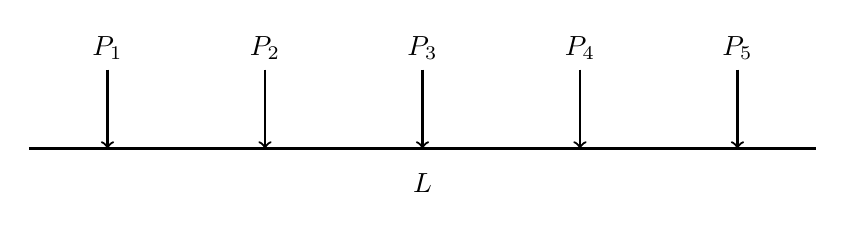
\begin{tikzpicture}

    % Draw the surface (flat beam)
    \draw[thick] (-5,0) -- (5,0); % Length L = 10 units

    % Label the surface as length L
    \node[below] at (0,-0.2) {$L$};

    % Define the locations of point loads (can be modified as needed)
    \def\pointLoadLocations{-4,-2,0,2,4} % x-coordinates of point loads
    \def\pointLoadLabels{} % Labels for point loads

    % Draw point loads
    \foreach \x [count=\i from 1] in \pointLoadLocations {
        % Draw the arrow for the point load
        \draw[->, thick] (\x, 1) -- (\x, 0);
        % Label the point load
        \node[above] at (\x, 1) {$P_\i$};
    }

\end{tikzpicture}
}
\end{center}
\paragraph{Distributed load} Load is distributed across $L$. it models the case where each load is infinitesimally small. 
\begin{center}
\resizebox{0.7\textwidth}{!}{ % Adjust the width to your preference
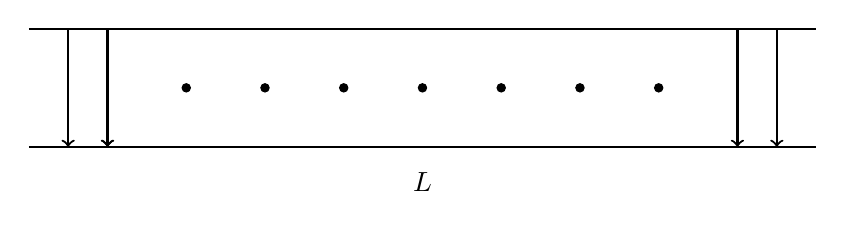
\begin{tikzpicture}

    % Draw the surface (flat beam)
    \draw[thick] (-5,0) -- (5,0); % Length L = 10 units
    \draw[thick] (-5,1.5) -- (5,1.5);

    % Label the surface as length L
    \node[below] at (0,-0.2) {$L$};

    % Define the locations of point loads (can be modified as needed)
    \def\pointLoadLocations{-4.5,-4,-4,4,4.5} % x-coordinates of point loads
    \def\pointLoadLabels{} % Labels for point loads

    % Draw point loads
    \foreach \x [count=\i from 1] in \pointLoadLocations {
        % Draw the arrow for the point load
        \draw[->, thick] (\x, 1.5) -- (\x, 0);
        % Label the point load
    }

    \foreach \x [count=\i from 1] in {-3,-2,-1,0,1,2,3} {
        % Draw the arrow for the point load
        \filldraw (\x,0.75) circle (1.5pt);;
        % Label the point load
    }
\end{tikzpicture}
}
\end{center}
When the load ($w$) is uniform across (\textbf{U}niformly \textbf{D}istributed \textbf{L}oad), the load  is calculated by:
\begin{equation}
    w = \frac{F}{L}
\end{equation}
\paragraph{Total Force due to Load} The load could be non-uniform. The total force is, in general:
\begin{equation}
    F=\int w dl
\end{equation}
the location of the force would be on the centroid (center of mass). Which is in the middle of \textbf{UDL}. In addition, for UDL, the total force is simply the area so:
\begin{equation}
    F= wL
\end{equation}
moreover, for non-UDL that increase/decrease linearly, it is the case of a \textbf{triangle} so:
\begin{equation}
    F= \frac{w_\text{max}L}{2}
\end{equation}
\section{Property of Materials}
\subsection{Stress and Strain}
\begin{center}
    \textit{"Stress and Strain are orthogonal - they are independent of each other''}
\end{center}
\begin{shaded}
\paragraph{Stress} ($\sigma$) is the distribution of applied force normalized on the plane. It is in the unit of MPa in CIV. Given by:
\begin{equation}\label{stress}
    \sigma = \frac{\Vec{F}}{A_\perp}
\end{equation}
Where:
    \begin{equation*}
    \begin{split}
    \Vec{F} = \text{Applied Force (MN)} \\
    A = \text{Cross section area normal to $\Vec{F}$ (m$^2$)} \\
    \end{split}
    \end{equation*}
\begin{note}
It is usually scaler considering uni-axial problems.
\end{note}
\end{shaded}
\begin{shaded}
    \paragraph{Strain} ($\epsilon$) is the unitless ratio between the material's actual length ($L$) and its change of length ($\Delta L$). Given by:
    \begin{equation}\label{strain}
        \epsilon = \frac{\Delta L}{L_0}
    \end{equation}
\begin{note}
Units of mm/m could also be used. $0.001=$1 mm/m is often an acceptable strain value in structures.
\end{note}
\end{shaded}
\paragraph{$\sigma$-$\epsilon$ Diagram} \textbf{Tensional stress} involves forces in opposite directions, which results in a strain. The relationship between stress and stress obeys \textbf{Hooke's law} at low stress and strain.
    \begin{equation}\label{sigmaepsilon}
        \sigma = E\epsilon
    \end{equation}
    Where:
    \begin{equation*}
    \begin{split}
    E = \text{\textbf{Young's Modulus}, the ratio between stress and stain} \\
    \end{split}
    \end{equation*}
so $\sigma$-$\epsilon$ diagram is linear when these two qualities are small and there are no effects of deformation. 
\begin{example}[Combined Stress-Stain Equation]
    Combining (\ref{sigmaepsilon}), (\ref{strain}) and (\ref{stress}), we have:
    \begin{equation}
        F = \frac{EA}{L}\Delta L
    \end{equation}
    And by Hooke's law, the spring constant, $k$, is 
    \begin{equation}
        k = \frac{EA}{L}
    \end{equation}
\end{example}
\subsection{Mild Steel}
\paragraph{Ductility} Ductile material could resist stress. It follows Hooke's law before it goes to a smaller strain-stress ratio. 
\paragraph{Brittle} Brittle material breaks at a certain lower level of stress-strain. 
\paragraph{Mild Steel} It follows a special stress-strain relationship. 
\begin{center}
\resizebox{0.7\textwidth}{!}{
\begin{tikzpicture}[scale=1.5]

    % Axis
    \draw[->] (0,0) -- (7,0) node[below] {Strain};
    \draw[->] (0,0) -- (0,5) node[left] {Stress};
    
    % Elastic region
    \draw[thick] (0,0) -- (2,3.5) node[midway, above left, font=\small] {Elastic Region};
    
    % Yield point
    \node at (2,3.5) [circle,fill=black,inner sep=1.5pt]{};
    \node[font=\small] at (-1,3.5) {Yield Stress ($\sigma_y$)};
    \draw[thick,dashed] (0,3.5) -- (2,3.5);
    
    % Yield plateau
    \draw[thick] (2,3.5) -- (4,3.5) node[midway, above, font=\small] {Yield Plateau};
    
     \draw[thick] (4,3.5) -- (5.5,4.5) node[midway, above] {Strain Hardening};
    
    % Necking and fracture
    \draw[dashed, thick] (5.5,4.5) -- (6.5,3.5) node[midway, right, font=\small] {Necking};
    
    % Labels
    \node[font=\small] at (5.7,4.7) {Ultimate Strength ($\sigma_u$)};
    
    % Ultimate stress point
    \node at (5.5,4.5) [circle,fill=black,inner sep=1.5pt]{};
    
    % Fracture point
    \node at (6.5,3.5) [circle,fill=black,inner sep=1.5pt]{};
    \node[font=\small] at (6.5,3.3) {Fracture};

\end{tikzpicture}
}
\end{center}
The stress-strain diagram has the following regions and properties.
\begin{enumerate}
    \item \textbf{Elastic Region} 
    \begin{itemize}
        \item Strains recoverable
        \item Linear, obeys Hooke's Law
    \end{itemize}
    \item \textbf{Yield Plateau Region}
    \begin{itemize}
        \item Non-recoverable strain
        \item Permanent damage
    \end{itemize}
    \item \textbf{Strain Hardening Region} Often ignored in design.
\end{enumerate}
\begin{note}
    There are two types of stress. The stress we would only discuss considers the original cross-section area, but true stress considers the current cross-section area. Ruptures occur when true stress is at a maximum, and that explains the decrease in stress in the necking region. 
\end{note}
\paragraph{Strain Energy} Is the area under the curve of a $\sigma-\epsilon$ diagram. It is in the unit of (MPa=MJm$^{-3}$).
\begin{equation}
    \int \sigma d\epsilon
\end{equation}
\paragraph{} For mild steel, the recoverable, elastic region is said to be the elastic strain energy. The non-revocable region is said to be the plastic strain energy.
\section{Oscillations}
\subsection{Dynamics in Single Degree of Freedom Systems}
\paragraph{Single Degree of Freedom Systems} Could be Subsets of the oscillation system
\begin{itemize}
    \item \textbf{Electrical}
    \item \textbf{Mechanical} $a\neq0$
    \item \textbf{Electromagnetic system}
\end{itemize}
\paragraph{Dynamic Equilibrium} D'Alembert's principle: An accelerating system may be placed in dynamic equilibrium by introducing and inertia for $F_i$ acting in the opposite direction to the acceleration. The have the following ODE:
\begin{align}
    0&=kx+m\ddot{x}\\\nonumber
    \Leftrightarrow x(t)&=A\sin(\omega_n+\phi)
\end{align} 
To verify, we have:
\begin{equation*}
    0 = A\sin(\omega_n+\phi)- mA\omega_n^2\sin(\omega_n+\phi)
\end{equation*}
That is true as per the natural frequency of vibration
\begin{equation}
    \omega_n=\sqrt{\frac{k}{m}}
\end{equation}
hence,
\begin{equation}
    f_n = \frac{1}{2\pi}\sqrt{\frac{k}{m}}
\end{equation}
\paragraph{Free Vibrations with Gravity} We have the rest displacement $\Delta_0=\frac{mg}{k}$
\begin{equation}
    x(t)=A\sin(\omega_n+\phi)+\Delta_0
\end{equation}
$k$ is not usually easy to find, so we can find frequency by  $\Delta_0=\frac{mg}{k}$
\begin{equation}
    f_n=\frac{1}{2\pi}\sqrt{\frac{g}{\Delta_0}}
\end{equation}
\section{Safety}
\begin{center}
    \textit{``The concept of safety is to avoid people getting hurt"}
\end{center}
\paragraph{Uncertainty Quantification} The measure of the significance of uncertainty, these could stem from:
    \begin{enumerate}
        \item Strength of Material and Geometry.
        \item Applied Load: Dead Load (unmovable) of Life Load (movable).
    \end{enumerate}
% APPENDIX
\paragraph{Evaluation of Safety} There are two main methods of determining the safety level:
\begin{enumerate}
    \item \textbf{Reliability} Risk, the probability of failure, multiplied by the consequences of failure.
    (Example) \textbf{Histograms of strength and load, risk related to overlapping region}
    \item \textbf{Working Stress/Allowable Stress Method} For factor of safety, we have
    \begin{equation}
        \text{Factor of safety (F.O.S)}=\frac{\text{Average Strength}}{\text{Average Applied Load}}
    \end{equation}
    In practice, to calculate allowable stress, we have:
    \begin{equation}
        \sigma_\text{allowable}=\frac{\sigma_y}{\text{F.O.S.}}
    \end{equation}
    Historically, F.O.S. is 10$\times$ during the 19$^\text{th}$ century. For example,
    \begin{itemize}
        \item \textbf{Brooklyn Bridge} (1800s): F.O.S. = 5.0$\times$.
        \item \textbf{Golden Gate Bridge} (1930s): F.O.S. = 2.6$\times$.
        \item \textbf{Akashi Kaikyo Bridge} (1998s): F.O.S. = 2.25$\times$.
    \end{itemize}
    F.O.S. decreases as we are more confident in our calculation. 
\end{enumerate}
\subsection{Structural Analysis}
\paragraph{Beam and Colume} Beam are horizontal and volume is vertical usually carrying axial load. 
\section{Design of Truss Bride}
\begin{center}
    \textit{``Strong, light, and stiff"}
\end{center}
\paragraph{Anatomy of Truss Bridge} See figure. MEmeber connects with joints (pin joints, hinge joints). 
\paragraph{}
\subsection{Moment of Inertia}
\begin{definition}[Curvature]
    Curvature $\phi$ [m$^{-1}$] is the measure of bentness between two ends $A$ and $B$, defined by:
    \begin{equation}
        \phi = \frac{\theta_A - \theta B}{L_0} = \frac{d \theta}{dx}
    \end{equation}
\end{definition}
    On the strain diagram plotted against depth, the angle is $\phi$, by the small angle approximation:
    \begin{equation}
        \phi = \frac{\epsilon_\text{top} - \epsilon_\text{bottom}}{h}
    \end{equation}
    Or we can use the relationship between $\phi$ and moment:
    \begin{equation}
        \phi =  \frac{M}{EI}
    \end{equation}
We have:
\begin{align*}
    \epsilon_i &= \phi y_i\\
    \sigma_i &= E\phi y_i\\
    F_i = E\phi y_i \Delta A
    \sum_i F_i = \sum_i E\phi y_i \Delta A
\end{align*}
\paragraph{First Moeenot of area} Since total force is zero, So we have:
\begin{equation}
    \phi E \int y dA = 0 
\end{equation}
The integral is known as the first moment of area. 
\begin{equation}
     \int y dA = 0 
\end{equation}
\paragraph{Stress and Bending Moment} The relation is given by the Navier's Equation. Since $\phi = \frac{\sigma}{Ey} = \frac{M}{EI}$, we have:
\begin{equation}
    \sigma = \frac{My}{I}
\end{equation}
\begin{shaded}
    \begin{equation}
        I = \iint y^2 dA
    \end{equation}
    Strain at a depth of $y$:
    \begin{equation}
        \epsilon_y = \phi y
    \end{equation}
    Moment:
    \begin{equation}
        M - EI\phi
    \end{equation}
    \begin{equation}
        I = \frac{bh^3}{12}
    \end{equation}
\end{shaded}
\subsection{Euler Buckling}
\paragraph{Buckling} Buckling is only possible in compression. The transition between axial shortening and buckling is said to be $P_\text{crit}$. It is important to prevent buckling as the structure fails without warning.
\begin{definition}[Elastic Buckling, Euler (1957)]
    Assume constant $E$ along the length, and $I$ is constant along the length. We have a pin at the top and bottom, that is, two ends can rotate. We also assume that the length is perfectly straight before buckling and we would use small angle approximation (since we only look at $P_\text{crit}$). \\
    \par Let $\Delta y$ be the horizontal distance of the bent. For small angle, we have
    $$
    \theta = \frac{\delta y}{\delta x} = \frac{y(L/2)}{L/2} 
    $$
    $$
        P_n = \frac{\pi^2 n^2 EI}{L^2}
    $$
    $$
        P_\text{crit} = \frac{\pi^2 EI}{L^2}
    $$
    $n$ is the count of the node in between the lenght
\end{definition}
\subsection{Curvature}
\paragraph{Curvature by 3 Method} Given $R$, the radius of the arc, the curvature
\begin{equation}
    \phi = 1/R
\end{equation}
\section{Wind}
\paragraph{Wind Bracing} 
\section{Virtual Work}
\paragraph{Work} In elastic deformation, for internal energy, we have
$$
W_\text{int} = V\frac{\sigma \epsilon}{2} = \frac{P\Delta}{2}
$$
In Hookes Law, for external energy, we have:
$$
W_\text{ext} = F\Delta r
$$
\paragraph{} For change of length, we have 
\begin{equation}
\Delta = \frac{PL}{EA}
\end{equation}
\paragraph{Deflection} To calculate the extension of the truss we can use a combined equation incorporating a virtual unit load $F^\star = 1$, and the equation $W_\text{ext} = W_\text{int}$
\begin{subequations}
    \begin{equation}
        \frac{1}{2}F_x\Delta x + \frac{1}{2}F_y\Delta y = \frac{1}{2}P_x\Delta x + \frac{1}{2}P_y\Delta y
    \end{equation}
    \begin{equation}
        \frac{1}{2}F^\star_x\Delta^\star x + \frac{1}{2}F^\star_y\Delta^\star y = \frac{1}{2}P^\star_x\Delta^\star x + \frac{1}{2}P^\star_y\Delta^\star y
    \end{equation}
    \begin{equation}
        (F^\star_x+F_x)(\Delta^\star x +\Delta x) + (F^\star_y+F_y)(\Delta^\star y +\Delta y) = (P^\star_x+P_x)(\Delta^\star x +\Delta x) + (P^\star_y+P_y)(\Delta^\star y +\Delta y)
    \end{equation}
\end{subequations}
Combining all three, after some algebra, we have:
\begin{equation}
    F^\star \Delta_{\hat{r}} = \sum^{i}P^\star_i \Delta_i
\end{equation}
\section{Vibraion}
\subsection{Free Vibration}
Since for change of length, we have:
\begin{align}
    \Delta = \frac{PL}{EA} \nonumber 
    \intertext{This could be rewritten as}
    P = \frac{EA}{L}\Delta \nonumber
    \intertext{For stiffness $k$, this could be molded as a simple harmonic motion with:}
    k = \frac{EA}{L}
\end{align}
\paragraph{} The solution to the differential equation $m\ddot{x} + k\dot{x} = mg$ is:
\begin{equation}
    x= A\sin{(\omega_nt + \phi)} + \Delta_0
\end{equation}
Where:
\begin{equation*}
\begin{split}
\omega_n = \sqrt{\frac{k}{m}}\text{, [rad s$^{-1}$] The natural frequency of vibration}\\
\Delta_0 =\text{Initial Displacement of the joint}
\end{split}
\end{equation*}
\paragraph{For Truss} We can use the method of virtual load to determine $\Delta_0$. 
\paragraph{Point Load} The natural frequency is \begin{equation}
\frac{15.76}{\sqrt{\Delta_0}}
\end{equation}
\paragraph{Uniform Load} The natural frequency is 
\begin{equation}
\frac{17.76}{\sqrt{\Delta_0}}
\end{equation}
\paragraph{Damping} Energy absorbed by friction, wind, etc.
\paragraph{} The differential equation for this is $m\ddot{x} + c\dot{x} + kx = mg$, where for some critical damping usually $\beta \in [0, 1 \text{ or } 2], c = 2\beta\sqrt{mk}$, for which the solution would be:
\begin{equation}
    x= A\sin{(\omega_n\sqrt{1-\beta}t + \phi)} + \Delta_0
\end{equation}
\subsection{Forced Vibration - Dynamic Amplification Factor} For some frequency of vibration $\omega$, the differential equation would be $m\ddot{x} + c\dot{x} + kx = mg + F_0\sin(\omega t)$
\begin{equation}
    x = \text{DAF} \frac{F_0}{k}\sin{(\omega t + \phi)}
\end{equation}
\paragraph{Dynamic Amplification Factor} Denoted as DAF, defined as
\begin{equation}
    \text{DAF} = \frac{1}{\sqrt{(1-(\frac{f}{f_n})^2)^2+ (2\beta \frac{f}{f_n})^2}}
\end{equation}
\section{Shear and Bending Moment} Consider a member AB with weight $w$, length $L$ and uniform load $P$ with a roller support on the left and a pin support on the right side. The member also has a constant axial force $N$. Let $N, V, M$ be the functions of axial force, sheer force and bending moment respectively w.r.t. $x$, the distance from left and right. We have, by equilibrium equations
\begin{subequations}
    \begin{equation}
        F_x: N(x) = N
    \end{equation}
    \begin{equation}
        F_y: V(x) = P + wx - Ay
    \end{equation}
    \begin{equation}
        M: M(x) = -\frac{wx^2}{2} - P(x-\frac{L}{2}) + xA_y
    \end{equation}
\end{subequations}
\paragraph{Relationship between $V$ and $M$}
\begin{subequations}
\begin{equation}
    V(x) = \frac{dM}{dX}
\end{equation}
\begin{equation}
    M(x) = \int_0^x V(x) dx
\end{equation}
\paragraph{Drawing Sheer Force Diagram} Imagine walking along and accumulating sheer force.
\paragraph{Drawing Bending Moment Diagram}  Imagine walking along and accumulating the area under the sheer force diagram. 
\paragraph{} Both graph at the end should add to zero. 
\end{subequations}
\subsection{Bending Movement and Stress}
\appendix
\def\thesection{\Alph{section}}
\newpage
\rhead{CIV Formula Booklet}
\lhead{\leftmark}
\pagenumbering{alph}

\section{Common Op-Amp Circuits} \label{app:OpAmpCircuits}
\begin{figure}[h!]
    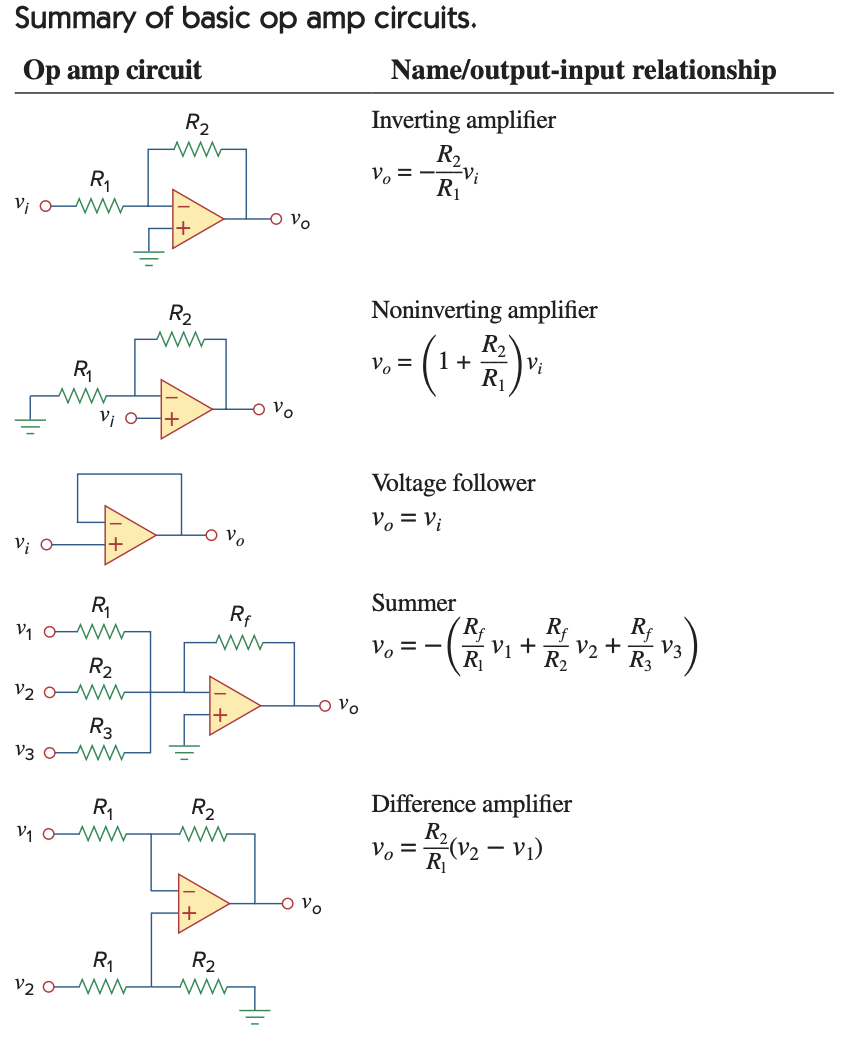
\includegraphics[width=0.9\linewidth]{AppendixItems/OpAmps.png}
    \centering
    \caption{Common Op-Amp Circuits}
\end{figure}
\end{document}